% Author: Izaak Neutelings (September 2020)
% Inspiration: https://tex.stackexchange.com/questions/25531/adding-underbrace-in-tikz
\documentclass[border=3pt,tikz]{standalone}
\usepackage{physics}
\usepackage{tikz}
\usetikzlibrary{calc} % for pic
\usetikzlibrary{arrows.meta}
\usetikzlibrary{patterns}
\usetikzlibrary{angles,quotes} % for pic
\tikzset{>=latex} % for LaTeX arrow head

\colorlet{myred}{red!65!black}
%\colorlet{mylightblue}{blue!20}
\colorlet{mydarkblue}{blue!30!black}
\colorlet{xcol}{blue!70!black}
\colorlet{vcol}{green!70!black}
\colorlet{acol}{red!50!blue!80!black!80}
\tikzstyle{ground}=[preaction={fill,top color=black!10,bottom color=black!5,shading angle=20},
                    fill,pattern=north east lines,draw=none,minimum width=0.3,minimum height=0.6]
\tikzstyle{mass}=[line width=0.6,red!30!black,fill=red!40!black!10,rounded corners=1,
                  top color=red!40!black!20,bottom color=red!40!black!10,shading angle=20]
\tikzstyle{vector}=[->,very thick,xcol,line cap=round]
\tikzstyle{force}=[->,myred,thick,line cap=round]
\tikzstyle{Fproj}=[force,myred!40]
\tikzstyle{mydashed}=[dash pattern=on 2pt off 2pt]
\tikzstyle{smallarrow}=[{Latex[length=2,width=2]}-{Latex[length=2,width=2]}]
\newcommand{\vbF}{\vb{F}}
\def\tick#1#2{\draw[thick] (#1) ++ (#2:0.1) --++ (#2-180:0.2)} %0.03*\xmax



\begin{document}


% WORK HORIZONTAL
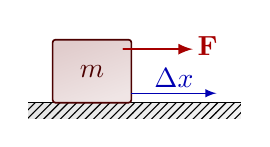
\begin{tikzpicture}
  \def\W{2.7} % ground width
  \def\D{0.2} % ground depth
  \def\h{0.8} % mass height
  \def\w{1.0} % mass width
  \draw[ground] (-0.3*\W,0) rectangle++ (\W,-\D);
  \draw (-0.3*\W,0) --++ (\W,0);
  \draw[mass] (-\w/2,0) rectangle++ (\w,\h) node[midway] {$m$};
  \draw[->,xcol] (\w/2,0.15*\h) --++ (0.4*\W,0) node[midway,above=-1.5] {$\Delta x$};
  \draw[force] (0.4*\w,0.85*\h) --++ (1.1*\h,0) node[above=1,right=-2] {$\vbF$};
\end{tikzpicture}


% WORK DIAGONAL
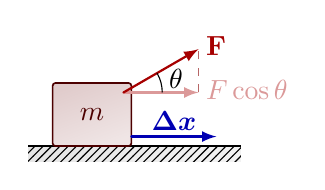
\begin{tikzpicture}
  \def\W{2.7}  % ground width
  \def\D{0.2}  % ground depth
  \def\h{0.8}  % mass height
  \def\w{1.0}  % mass width
  \def\F{1.1}  % force magnitude
  \def\ang{30} % angle force
  \coordinate (F0) at (0.4*\w,0.85*\h);
  \coordinate (Fx) at ($(F0)+({\F*cos(\ang)},0)$);
  \coordinate (F)  at ($(F0)+(\ang:\F)$);
  \draw[ground] (-0.3*\W,0) rectangle++ (\W,-\D);
  \draw (-0.3*\W,0) --++ (\W,0);
  \draw[mass] (-\w/2,0) rectangle++ (\w,\h) node[midway] {$m$};
  \draw[force,xcol] (\w/2,0.15*\h) --++ (0.4*\W,0) node[midway,above=-1.5] {$\vb*{\Delta x}$};
  \draw[dashed,myred!80!black!60] (Fx) -- (F);
  \draw[Fproj] (F0) -- (Fx) node[above=1,right=-1] {$F\cos\theta$}; %\vu{x}
  \draw[force] (F0) -- (F)  node[above=1,right=-1] {$\vbF$};
  \draw pic["$\theta$",draw=black,angle radius=14,angle eccentricity=1.4] {angle=Fx--F0--F};
\end{tikzpicture}


% WORK DIAGONAL - negative
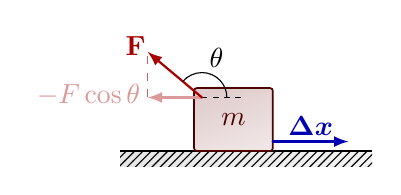
\begin{tikzpicture}
  \def\W{3.2}   % ground width
  \def\D{0.2}   % ground depth
  \def\h{0.8}   % mass height
  \def\w{1.0}   % mass width
  \def\F{0.9}   % force magnitude
  \def\ang{140} % angle force
  \coordinate (F0) at (-0.4*\w,0.85*\h);
  \coordinate (Fx) at ($(F0)+({\F*cos(\ang)},0)$);
  \coordinate (F)  at ($(F0)+(\ang:\F)$);
  \draw[ground] (-0.45*\W,0) rectangle++ (\W,-\D);
  \draw (-0.45*\W,0) --++ (\W,0);
  \draw[mass] (-\w/2,0) rectangle++ (\w,\h) node[midway] {$m$};
  \draw[dashed,myred!80!black!60] (Fx) -- (F);
  \draw[force,xcol] (\w/2,0.15*\h) --++ (0.3*\W,0) node[midway,above=-1.5] {$\vb*{\Delta x}$};
  \draw[Fproj] (F0) -- (Fx) node[above=1,left=-1] {$-F\cos\theta$}; %)\vu{x}
  \draw[mydashed] (F0) --++ (0.5*\w,0) coordinate (R);
  \draw[force] (F0) -- (F) node[above=2,left=-3] {$\vbF$};
  \draw pic["$\theta$",draw=black,angle radius=9,angle eccentricity=1.7] {angle=R--F0--F};
\end{tikzpicture}


% HORIZONTAL ground - lift
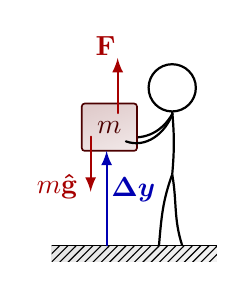
\begin{tikzpicture}
  \def\W{2.1}  % ground width
  \def\D{0.2}  % ground depth
  \def\h{0.6}  % mass height
  \def\w{0.7}  % mass width
  \def\H{2.0}  % human height
  \def\F{0.7}  % human height
  \def\mx{-0.15*\W} % mass x coordinate
  \def\my{ 0.60*\H} % mass y coordinate
  
  % PERSON
  \draw[thick] (0.23*\W,\H) circle (0.3) coordinate (H);
  \draw[thick] (H)++(-90:0.3) coordinate (N) to[out=-85,in=85]++ (0,-0.40*\H) coordinate (P);
  %\draw[thick,line cap=round] (N)++(-85:0.03) to[out=-115,in=3] (RH);
  \draw[thick,line cap=round] (N)++(-85:0.03) to[out=-120,in=-10] (\mx+0.3*\w,\my+0.3*\h); % right arm
  \draw[thick] (P) to[out=-110,in=85] (0.15*\W,0); % right leg (on the left)
  \draw[thick] (P) to[out=-80,in=108] (0.29*\W,0); % left leg (on the right)
  
  % SETUP
  \draw[ground] (-\W/2,0) rectangle++ (\W,-\D);
  \draw (-\W/2,0) --++ (\W,0);
  \draw[mass] (\mx-\w/2,\my) rectangle++ (\w,\h) node[midway] {$m$};
  \draw[thick,line cap=round] (N)++(-85:0.03) to[out=-110,in=-20] (\mx+0.3*\w,\my+0.2*\h); % right arm
  
  % FORCES
  %\draw[->] (0.42*\W,0.5*\h) --++ (0,0.9*\h) node[below=4,right=0] {$y$};
  \draw[force] (\mx+0.15*\w,\my+0.8*\h) --++ (0, \F) node[above left=-3] {$\vbF$};
  \draw[force] (\mx-0.34*\w,\my+0.3*\h) --++ (0,-\F) node[below=-2,left=1] {$m\vu{g}$};
  \draw[force,xcol] (\mx-0.05*\w,0) --++ (0,\my) node[midway,above=3,right=-2] {$\vb*{\Delta y}$};
  
\end{tikzpicture}


% WORK diagram
\def\xmax{3}
\def\ymax{2.2}
\begin{tikzpicture}
  \def\x{.15*\xmax}
  \def\dx{.65*\xmax}
  \def\F{.77*\ymax}
  
  % AREA
  \coordinate (A) at (\x,\F);
  \coordinate (B) at (\x+\dx,\F);
  \fill[xcol!20] (\x,0) rectangle++ (\dx,\F) node[midway,blue] {$W$};
  
  % LINE
  \draw[very thick,xcol] (A) -- (B);
  \fill[xcol] (A) circle (0.04); %node[right=5,above=2] {$P_1$, $V_1$};
  \fill[xcol] (B) circle (0.04); %node[right=2] {$P_2$, $V_2$};
  
  % AXIS
  \draw[->,thick] (0,-0.1*\ymax) -- (0,\ymax); %node[left] {$F$};
  \draw[->,thick] (-0.1*\xmax,0) -- (\xmax,0) node[below] {$x$};
  \tick{\x,0}{90} node[below] {$x_1$};
  \tick{\x+\dx,0}{90} node[below] {$x_2$};
  \tick{0,\F}{0} node[left] {$F$};
  \draw[<->] (\x,1.15*\F) --++ (\dx,0) node[midway,above=-3,fill=white,inner sep=0] {$\Delta x$};
  
\end{tikzpicture}


% WORK diagram - curve
\def\xmax{3.4}
\def\ymax{2.2}
\begin{tikzpicture}
  \def\x{.58*\xmax}
  \def\dx{.07*\xmax}
  \def\F{.75*\ymax}
  
  % AREA
  \coordinate (Ax) at (.12*\xmax,0);
  \coordinate (Cx) at (.84*\xmax,0);
  \coordinate (A) at (.12*\xmax,.55*\ymax);
  \coordinate (B) at (.48*\xmax,.80*\ymax);
  \coordinate (C) at (.84*\xmax,.60*\ymax);
  \fill[xcol!20] (A) to[out=10,in=180] (B) to[out=0,in=170] (C) |- (Ax) -- cycle;
  \path (Ax) -- (C) node[midway,left=-2,blue] {$W$};
  
  % LINE
  \draw[very thick,xcol] (A) to[out=10,in=180] (B) to[out=0,in=170] (C);
  \fill[xcol] (A) circle (0.04); %node[right=5,above=2] {$P_1$, $V_1$};
  \fill[xcol] (C) circle (0.04); %node[right=2] {$P_2$, $V_2$};
  
  % AXIS
  \draw[->,thick] (0,-0.1*\ymax) -- (0,\ymax); %node[left] {$F$};
  \draw[->,thick] (-0.1*\xmax,0) -- (\xmax,0) node[below] {$x$};
  \tick{Ax}{90} node[below] {$x_1$};
  \tick{Cx}{90} node[below] {$x_2$};
  \tick{0,\F}{0} node[left] {$F$};
  
  % RECTANGLE
  \draw[dashed] (0,\F) --++ (\x,0);
  \draw[xcol] (\x,0) rectangle++ (\dx,\F);
  \draw[smallarrow] (\x,-0.08) --++ (\dx,0) node[midway,below=0,scale=0.9] {$\dd{x}$};
  %\node[below=-1] at (\x+\dx/2,0) {$\Delta x$};
  
\end{tikzpicture}



\end{document}